\documentclass{standalone}
\usepackage{tikz}

\begin{document}

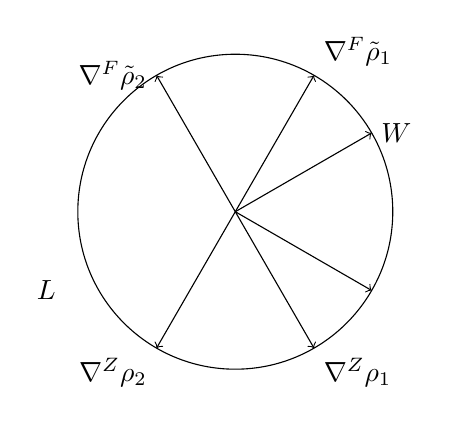
\begin{tikzpicture}[scale=2]
    % Draw the circle
    \draw (0,0) circle (1);
    
    % Label the circle
    \node at (-1.2, -0.5) {$L$};
    
    % Draw the vectors
    \draw[->] (0,0) -- (0.866, 0.5) node[right] {$W$};
    \draw[->] (0,0) -- (0.866, -0.5);
    \draw[->] (0,0) -- (0.5, 0.866) node[above right] {$\nabla^F \tilde{\rho}_1$};
    \draw[->] (0,0) -- (0.5, -0.866) node[below right] {$\nabla^Z \rho_1$};
    \draw[->] (0,0) -- (-0.5, 0.866) node[left] {$\nabla^F \tilde{\rho}_2$};
    \draw[->] (0,0) -- (-0.5, -0.866) node[below left] {$\nabla^Z \rho_2$};
\end{tikzpicture}

\end{document}